\input{header.tex}
% this file declares acronyms. There are two classes: abbrev for abbreviations and nomencl for nomenclature

\acsetup{
  first-style=short
}

% class `abbrev': abbreviations:
\DeclareAcronym{CE}{
  short = CE ,
  long  = contractile element ,
  class = abbrev
}
\DeclareAcronym{SEE}{
  short = SEE ,
  long  = serial elastic element ,
  class = abbrev
}
\DeclareAcronym{PEE}{
  short = PEE ,
  long  = parallel elastic element ,
  class = abbrev
}
\DeclareAcronym{SDE}{
  short = SDE ,
  long  = serial damping element ,
  class = abbrev
}
\DeclareAcronym{MTU}{
  short = MTU ,
  long  = muscle tendon unit ,
  class = abbrev
}

% class `nomencl': nomenclature
\DeclareAcronym{angelsperarea}{
  short = \ensuremath{a} ,
  long  = The number of angels per unit area ,
  sort  = a ,
  class = nomencl
}
\DeclareAcronym{numofangels}{
  short = \ensuremath{N} ,
  long  = The number of angels per needle point ,
  sort  = N ,
  class = nomencl
}
\DeclareAcronym{areaofneedle}{
  short = \ensuremath{A} ,
  long  = The area of the needle point ,
  sort  = A ,
  class = nomencl
}

% usage: \ac{ny}, \ac{la} and \ac{un} are abbreviations 
%        whereas \ac{angelsperarea}, \ac{numofangels} and \ac{areaofneedle} are part of the nomenclature


\graphicspath{
{images/summer_school_study/png/}
{images/summer_school_study/}
{images/summer_school_study/plots/}
{images/summer_school_study/2018/}
{images/fiber_creation/}
}

\begin{document}

%\setcounter{tocdepth}{2}
\tableofcontents
%\newpage


\part{Introduction}
%  \chapter{Motivation}
%  - great picture, digital human vision, connection to soft tissue robotics\\
%  - EMG, parameter estimation, see motivation of IRTG paper\\
%  - MU estimation\\
%  
%  \chapter{State of the art and aims}
%  \chapter{Own contributions}
%  - own contributions
%  \chapter{Overview}
%  - structure of following sections
\part{Digital human}

%\input{02_comparative_study}

% \chapter{Formulation of electrophysiology and muscle contraction}
%    - electrophysiology introduction
%    \section{State of the art}
%    - Hodgkin-Huxley, shorten, advanced models, how it gets solved
%    \section{discretization}
%    - discretization of electrophysiology, operator splitting
%    \section{Standard for formulation of models}
%    - cellml introduction
%    \section{Bidomain}
%    - EMG
%    \section{Multidomain}
%    - multidomain formulation
%    \section{Formulation of solid mechanics}
%    - basics solid mechanics framework, material modeling, 
%    
%    \section{Simulation workflow}
%    - simulation workflow of skeletal muscle
%  
% \chapter{Numerics}
%   \section{Fundamentals of the discretization}
%    \section{Finite element method}
%    - basics FEM formulation of Laplace operator and diffusion equation, boundary conditions
%    \section{Incompressible nonlinear solid mechanics}
%    - incompressibility, penalty formulation vs. mixed formulation\\
%    - governing nonlinear eq.\\
%    - jacobian
%   \section{Numerical schemes}
%    \section{time stepping schemes}
%    \section{linear system solvers}
%    \section{newton algorithm}
%  % 
% \chapter{Simulation software}
%    \section{State of the art}
%    - review on bioengineering simulation frameworks 
%    
%    \section{OpenCMISS}
%  - OpenCMISS introduction, iron zinc cmgui, unstructured\\
%  
%  - Strang splitting, solvers 1D\\
%  - improved interpolation\\
%  - parallelization, issue with 1D \\
%  - 3D parallelization strategies\\
%  - design flaws, memory\\
%    % untergliedern, z.B. schnittstellen parall etc.
%    \section{The simulation framework \emph{opendihu}}
%    - modularity of opendihu, concepts (python c++ build system)
%    \section{Overview of discretization features}
%    - feature overview, implemented equations, ansatz functions, meshes
%    \section{Input and output}
%    - file i/o parallel, i: only local data important for high parallelism, o: paraview
%    \section{In-situ visualization}
%    - in-situ
%    \section{Details on the implementation}
%    \section{Representation of structured meshes}
%    \section{Parallel data handling}
%    - data structures, petsc variables, partitioning, ghost communication
%    \section{Implementation of boundary conditions}
%    - Neumann, Dirichlet boundary conditions
%    \section{Implementation of material formulation and automatic derivation of derivatives}
%    - implementation of solid mechanics with analytic differentiation
%    
%    \section{efficient and configurable data transfer}
%    - data layout details, efficient transfer of variables between solvers
%    \section{Mapping between meshes}
%    - parallel mapping between meshes, invertability of index space represesantion
%    \section{An efficient solver to the Monodomain equation}    
%    - cellml code generator and its optimizations - openmp, simd, vc
%    \section{Details on the partitioning}
%    - fibers emg structure and partitioning
%    \section{Parallelization of the multidomain system}
%    - multidomain parallelization, reordering of matrix
%    \section{load balancing}
%    - load balancing on fiber level
% \chapter{External coupling}
%    - introduction to external coupling, precice
%    \section{coupling with FEBio}
%    \section{coupling with AceFEM}
%  
\chapter{Generation of Meshes}

The formulations of electrophysiology and contraction of tendon and muscle tissue are given on different domains.
The muscle belly forms the domain $\Omega_M$. A layer of fat and skin tissue on top of the muscle is denoted the body domain $\Omega_B$.
On both longitudinal ends, the muscle is attached to tendons, given by the domains $\Omega_{T,1}$ and $\Omega_{T,2}$.

All these domains are placed in the 3D Euclidean space, $\Omega_M,\Omega_B,\Omega_{T,i} \subset \R^3$.
Additionally, formulation of electrophysiology on individual muscle fibers need one-dimensional domains $\Omega_{F,i} \subset \R^3$ for $i \in \{0,\dots,n_f\}$. In such formulation, the whole muscle typically consists of a large number $n_f$ of these fiber domains.
Each domain $\Omega_{F,i}$ is a 1D manifold embedded in the 3D domain. The domains are visualized in \cref{fig:fibers_domains}.

\begin{figure}%
    \centering%
    \def\svgwidth{8cm}%
    \input{images/fiber_creation/domains.pdf_tex}%
    \caption{Visualization of the computational domains: tendons $\Omega_{T,1}, \Omega_{T,2}$, muscle belly $\Omega_M$, body domain $\Omega_B$ and fiber domains $\Omega_{F,i}$.}%
    \label{fig:fibers_domains}%
\end{figure}%

For discretization using the Finite Element Method, we approximate the 3D domains and 1D manifolds, $\Omega_\text{3D}$ and $\Omega_\text{1D}$, 
by a number of 3D elements $\{U_{\text{3D},i}\}_{i=1,\dots,n}$ with $U_{\text{3D},i} \subset \R^3$, respective 1D elements $\{U_{\text{1D},i}\}_{i=1,\dots,n}$, with $U_{\text{1D},i}\subset \R^3$.
An element is given by a number of nodes and their connectivity information. Their disjoint union approximates the overall computational domain,
 $\dot{\bigcup}_{i=1}^{n} U_\text{3D} \approx \Omega_\text{3D}$ and $\dot\bigcup_{i=1}^{n} U_\text{1D} \approx \Omega_\text{1D}$.

The elements can be defined by a mesh. In this section, structured meshes are assumed. 
A 3D structured mesh is homomorphic to a 3D regular cartesian grid. 
The number $n$ of elements is the product of the numbers $n_i, n_j$ and $n_k$ of elements in the three coordinate directions $x,y$ and $z$ of the regular cartesian grid,
 i.e., $n = n_i\,n_j\, n_k$.
Each element can be indexed by a triple $(i,j,k)$ of indices with the ranges $i \in \{0,\dots,n_i-1\}, j \in \{0,\dots, n_j-1\}$ and $k \in \{0,\dots,n_k-1\}$. 
In the program, typically, consecutive indices $\iota$ are used that iterate over all elements $\iota \in \{0,\dots,n-1\}$ and are obtained from the index triples by the mapping 
$(i,j,k) \mapsto \iota = k\,n_i\,n_j + j\,n_i + i$.

The elements can have different numbers of nodes, depending on the spatial order of consistency of the discretization. 
In this section, only 1D elements with two nodes and quadrilaterial 3D elements with $2^3=8$ nodes are considered. 
Higher order elements can be composed geometrically by using the nodes of the respective number of adjacent elements in the structured mesh.
For this purpose, we always generate 3D meshes with an uneven number of elements in the coordinate directions. 
Thus, linear elements with eight nodes or quadratic elements with 27 nodes can be created from the same global set of nodes.

In the following, algorithms for the generation of the needed meshes are presented. 
The requirement is to construct a 3D structured mesh that fills a given volume. This is needed for the muscle and tendon domains, $\Omega_M$ and $\Omega_{T,i}$.
Additionally, for the 3D muscle domain, a specified number of 1D muscle fiber meshes that are embedded in the 3D mesh have to be created. 
The fibers should be positioned to match the anatomy of the muscle. For the biceps and triceps muscles with their fusiform layout,
a streamlined orientation of the fibers is needed.

% overview subsections

\section{Related Works}

\section{Preprocessing of the Muscle Geometry}

The first step towards creating a structured mesh is to obtain a representation of the surface of the muscle. 
Starting point is a human biomedical imaging data set. In this section, two possible workflows are presented how to extract the muscle and tendon surface. 
The two workflows are visualized in \cref{fig:scheme_preprocessing}. The workflow using the branch on the left side in \cref{fig:scheme_preprocessing} is automized but only works for the particular data set and extracting the biceps muscle.
The right branch involves manual steps and is applicable for any muscle geometry.

% overview over subsections

\begin{figure}%
  \centering%
  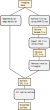
\includegraphics[height=15cm]{images/fiber_creation/scheme_preprocessing.pdf}%
  \caption{Workflow of generating a surface representation of the muscle and tendons from imaging data. Intermediate results are visualized as yellow boxes. Two possible branches are shown. On the left, the imaging data is processed using automatic processing to directly retrieve points on the surface of the muscle. On the right, the same is achieved with three steps of which the first one involves manual adjustments. At the end, a spline surface smooths the collected data from both possibilities to yield the resulting surface representation.}%
  \label{fig:scheme_preprocessing}%
\end{figure}%

\subsection{Data source}
Anatomic images provide the basis for the extraction of muscle geometries.
The used data set originates from the Visible Human Project \cite{visible_human_male} of 
the United States National Library of Medicine. 
The project has published anatomic images derived from a male cadaver, among other data sets.
The data, known as \say{Visible Human Male}, were published in 1994.
Colored images of transversal cross sections were obtain by cryosectioning.
A total of \num{1871} images with dimensions of \num{2048} by \num{1216} pixels and 24 bit color depth visualize the whole human body. Parts of the upper arms are contained in approximately 500 of these images. The size of a pixel is \SI{0.33}{\milli\meter} in transversal direction and \SI{1}{\milli\meter} in axial direction. The size of the complete set of JPEG compressed images is \SI{772}{\mega\byte}. Cropping and selecting the relevant portions of the upper arm extracts a dataset with the size of \SI{35}{\mega\byte}.

An extract of an image of the upper arm is given in \cref{fig:vhp_image}. 
Biceps and triceps brachii muscles can be identified as the dark red tissue. For the biceps, the two muscle heads are visible, separated by the bright diagonal line from bottom left to top right. For the triceps, at least two of the three heads can be identified. The blue background is colored frozen gelatin that was needed during cryosection to stabilize the arms.

\begin{figure}%
  \centering%
  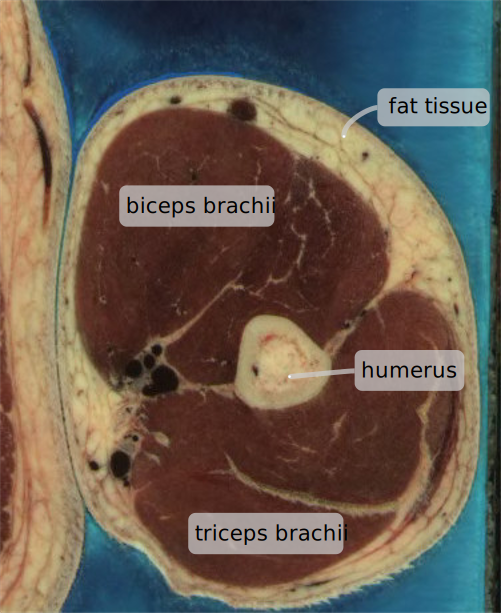
\includegraphics[height=10cm]{images/fiber_creation/vhp.png}% 0483
  \caption{Exemplary extract of image number 483 from the Visible Human Male. A transversal slice of the left upper arm is shown as seen from the bottom. The biceps and triceps muscles as well as the humerus bone can be identified. }%
  \label{fig:vhp_image}%
\end{figure}%

\subsection{Automatic surface extraction}
This section outlines the automatic algorithm to obtain the muscle surface from the Visible Human Male data set. The scheme corresponds to the left branch in \cref{fig:scheme_preprocessing}. The algorithm was implemented as Python script as part of the Bachelor thesis of Kusterer \cite{Kusterer} that was supervised by me.
The algorithm is capable of extracting muscle and bone geometries from the described imaging data.

At first, the color values of the images are used to segment the imaging data into muscle tissue, surrounding tissue and skeletal structure. The algorithm traverses the selected and cropped relevant parts of the images. For example, to segment the biceps muscle, the image region of pixels coordinates $(x,y)$ with $x \in [1300,1720] $ and $ y\in[1030,1720]$ are considered in the images with numbers 284 to 778. 

For every such part of an image, pixels that match a certain range in the RGB color space are marked and categorized. The categories are muscle tissue and, for comparison, also bone tissue. The corresponding color ranges are given in \cref{tab:color_ranges}.
This color based classification does not succeed everywhere as the white shade corresponds not only to bone material but also to fat and other tissue. Therefore, the algorithm removes artifacts located near the outer gelatine from the set of pixels categorized as bone. 

\begin{table}
  \centering%
  \begin{tabular}{l|lll}
    \hline
    & red & green & blue\\
    \hline
    muscle & $60 - 100$& $30-75$   & $15-60$\\
    bone   & $145-255$ & 1$35-205$ & $60-160$\\
    \hline
  \end{tabular}
  \caption{Ranges in the RGB color space to identify pixels of muscle and bone segments. The numbers correspond to 24 bit colors with the range $[0,255]$ for every color channel.}%
  \label{tab:color_ranges}%
\end{table}

Exemplary results for image number 483 are given in the left column of \cref{fig:vhp_image}.
It can be seen that the marked regions for muscle and bone have gaps in the interior resulting from differently colored tissue inside muscles and bones. On some images, the set of pixels also includes small objects outside the actual muscle and bone regions.

To reduce the gaps and small objects, the morphological operations \emph{closing} and \emph{opening} are performed on the data. These operations consist of \emph{dilation} and \emph{erosion} steps. Both are pixel based operations that traverse the dataset and for every pixel consider a window of $3\times 3$ pixels centered at the current position. Dilation picks the maximum value and erosion the minimum value from this window and assigns it as the pixel's value in a new image. In our case, values of zero and one correspond to non-categorized and categorized pixels, respectively.

Closing consists of dilation followed by erosion and closes small gaps or holes in the marked objects. Opening consists of erosion followed by dilation and removes small artifacts outside the actual bone and muscle areas. It was found effective to perform each dilation and erosion twice in sequence to yield good results with almost no more holes and unwanted small objects.

Next, the algorithm determines the contours of all regions with marked pixels. This leads to lines with a width of one pixel that enclose the muscle and bone areas. The right column of \cref{fig:extraction} shows the results after this step. It can be seen that the morphological operations close numerous gaps. In some images, as in the considered example, the muscle area gets split into multiple smaller enclosed regions which is not desired. However, proper contours of the biceps are found in the majority of images. 

\fboxsep=0mm   % padding thickness
\fboxrule=1pt   % border thickness
\begin{figure}%
  \centering%
  \fcolorbox{black}{black}{\includegraphics[height=7cm,trim=0 0 0 6cm, clip]{images/fiber_creation/extraction_segmentation_482.png}}\quad%
  \fcolorbox{black}{black}{\includegraphics[height=7cm,trim=0 0 0 4cm, clip]{images/fiber_creation/extraction_contour_482.png}}\vspace*{5mm}\\
  \fcolorbox{black}{black}{\includegraphics[height=7cm,trim=0 0 0 6cm, clip]{images/fiber_creation/extraction_bone482.png}}\quad%
  \fcolorbox{black}{black}{\includegraphics[height=7cm,trim=0 0 0 6cm, clip]{images/fiber_creation/extraction_surface_bone482.png}}%
  \caption{Intermediate steps of the algorithm to determine surface geometry of muscles and bones. The left columns shows pixels from the image in \cref{fig:vhp_image} that were categorized to be muscle tissue (top) and bone material (bottom). The right column shows a later step in the algorithm, where the surface of muscle (top) and bone (bottom) is estimated.}%
  \label{fig:extraction}%
\end{figure}%

In the next step, a single contour for each of muscle and bone is obtained in every image. If there are multiple contours per image, the one that is located the most in upper right location within the image is selected for the muscle. If all contours in an image are shorter than 20 pixels, this is a sign of bad segmentation quality and the whole image gets discarded.

The result is a set of contours for muscle and bone in the cross-sectional planes of the images. Combining these, we get a point cloud in 3D space that approximates the surface of the biceps muscle and the surfaces of the considered bones humerus, ulna and radius. Using these points, a spline surface can be fitted and subsequently triangulated. Resulting surfaces for the biceps and humerus bones are shown in \cref{fig:extraction_result}.
%
\begin{figure}%
  \centering%
  \begin{subfigure}[t]{0.48\textwidth}%
    \centering%
    \includegraphics[height=6cm]{images/fiber_creation/extraction_biceps.png}%
    \caption{Surface of the biceps brachii muscle. At the right side of the muscle, the groove of the humerus bone can be seen.}%
    \label{fig:extraction_result_biceps}%
  \end{subfigure}
  \begin{subfigure}[t]{0.48\textwidth}%
    \centering%
    \includegraphics[height=6cm]{images/fiber_creation/extraction_humerus00.png}%
    \caption{Surface of the humerus}%
    \label{fig:extraction_result_humerus}%
  \end{subfigure}    
  \caption{Resulting surfaces of biceps and humerus bone obtained by the automatic surface extraction algorithm.}%
  \label{fig:extraction_result}%
\end{figure}%

The runtime for the algorithm is \SI{121}{\minute} on a AMD Ryzen 5 1600 processor with 6 cores, 3.2 GHz and \SI{16}{\giga\byte} RAM, of which a maximum of \SI{2}{\giga\byte} was used at maximum. Because processing of the images can be done in parallel, the runtime can be reduced to approximately half (\SI{62}{\minute}) using 2 threads and to a quarter (\SI{30}{\minute}) using 6 threads.

The advantage of the presented algorithm is that the outcome solely depends on the imaging data and, thus, no modeling error by manual approximation of the geometry occurs. For example, the obtained surfaces of biceps and humerus geometrically fit perfectly into each other. Intermediate steps are stored as black and white images. By editing these between the steps of the algorithm, manual tweaking is possible and could lead to increased quality of the results.

A disadvantage is that it relies on color information in the imaging data to differentiate between muscle and other tissue. Because the involved tissue has similar colors, these differences are often small. Furthermore, the color ranges need to be determined experimentally. Therefore, the algorithm is not very robust with respect to image noise and needs adjustments when it should be used to extract other muscles. Expert knowledge about the location and shape of human muscles cannot be used easily to improve the results of the algorithm.

A different approach is to manually segment the imaging data and construct surfaces with the help of a tool. This approach is described in the following section.

\subsection{Manually guided surface extraction}\label{sec:surf_extr}

The manually guided segmentation is done using the \emph{MAP client} of the Musculoskeletal Altas Project (MAP) \cite{mapclient}. This application allows to create and execute a workflow to achieve data processing and simulation tasks. In a graphical window, the user can place and connect various workflow steps. When executing the workflow, each step shows a dialog where the required configuration can be entered or the operations can be performed on a visual presentation of the data at this workflow stage. 

Possible workflow steps include source and sink operations such as reading image data and writing meshes. Imaging data such as the 2D images from the Visual Human Male can be visualized in a 3D representation. The user can place points in the 3D space and try to match borders of the muscles and structures to extract from the data.
Further workflow steps allow to create meshes of predefined geometrical shapes, such as cubes and cylinders and merge them into a common mesh. These meshes can be fitted to point clouds of user defined points. This is done by a least squares approach minizing the distances between user created points and the mesh surface.

The MAP client has a plugin architecture and allows to create new workflow steps. It includes features from OpenCMISS, especially data processing formats and tools from OpenCMISS Zinc. Meshes can be created with 3D cubic Hermite elements that allow a high geometric modelling flexibility with a low number of nodes. Such meshes are stored in the OpenCMISS file format of \code{exnode} and \code{exelem} files.

As a result, meshes of individual muscles or the whole human organism can be created. \Cref{fig:vhp_geometry} shows meshes that were create from the cryosectioning data of the Visible Human Male. In \cref{fig:vhp_total} almost the whole body has been extracted. In \cref{fig:vhp_detail}, the mesh consisting of cubic Hermite elements is visualized. A relatively coarse mesh width suffices to model a smooth surface of the body. When exported in the exfiles format from the MAP client, the data can be visualized, e.g., using \emph{cmgui}, the visualization tool of OpenCMISS Zinc.

\begin{figure}%
  \centering%  
  \begin{subfigure}[t]{0.48\textwidth}%
    \centering%
    \includegraphics[height=10cm]{images/fiber_creation/skin00.png}%
    \caption{Mesh of the trunk and limbs, surface has been triangulated for visualization.}%
    \label{fig:vhp_total}%
  \end{subfigure}
  \quad
  \begin{subfigure}[t]{0.48\textwidth}%
    \centering%
    \includegraphics[height=7cm]{images/fiber_creation/elements4.png}%
    \caption{Detail view of part of the right upper arm and the trunk with blue nodes and contours of a mesh with cubic Hermite elements.}%
    \label{fig:vhp_detail}%
  \end{subfigure} 
  \caption{Mesh of the Visible Human Male from the Visible Human Project.}%
  \label{fig:vhp_geometry}% 
\end{figure}%

The mesh width of the meshes obtained using the MAP client was chosen such that the surface fitting yielded good results. The meshes are not necessarily ready for use in a simulation, especially if a  high mesh resolution is desired. 
Apart from the mesh width also the type of elements can be different than what is needed for a Finite Element simulation. Our goal is to obtain meshes with linear or quadratic Lagrange elements with configurable mesh widths for the specified upper arm muscles, such as the biceps brachii.

Therefore, the next step of the workflow, as visualized by the right branch of \cref{fig:scheme_preprocessing}, is to transform the volume mesh into a surface mesh which then can be used as basis for further meshing. This is visualized with the example of the biceps muscle in \cref{fig:biceps_processing}. The basis is the Hermite mesh shown in the left-most image.

\begin{figure}%
  \centering%
  \includegraphics[height=10cm]{images/fiber_creation/exfile.png}\quad%
  \includegraphics[height=10cm]{images/fiber_creation/biceps23.png}%
  \includegraphics[height=10cm]{images/fiber_creation/biceps22.png}%
  \includegraphics[height=10cm,trim=-2cm 0 0 -2cm, clip]{images/fiber_creation/splines00.png}%
  \caption{Processing the geometry of the biceps brachii muscle. From left to right: mesh with cubic Hermite elements, STL mesh with inside triangles, STL surface mesh where triangles lying inside have been removed, Spline surface of the muscle belly.}%
  \label{fig:biceps_processing}%
\end{figure}%

The Hermite elements can be triangulated and stored as an STL file using the tool \code{cmgui}. This process triangulates the non-planar faces of all Hermite elements. This leads to a dataset with triangles on the surface and in the inside of the volume, as can be seen in the second image of \cref{fig:biceps_processing}. At this stage, the use of the MAP and OpenCMISS related tools is finished and further processing steps are performed using tools from opendihu that we developed on our own.

A Python script removes the triangles in the inside of the volume. The detection whether a triangle is inside the volume is done by casting four rays from the center of gravity of the triangle and determining if the rays intersect any other triangles. The rays have directions $(x,y,z) = (\pm1,\pm1,\frac13)$, where the $z$ axis is oriented along the muscle and the $x$ and $y$ are oriented in radial direction. The ray-triangle intersection is done using the fast Möller-Trumbore algorithm \cite{ray-triangle}. For every ray, all triangles are checked.
Only if all four rays intersect at least one more triangle, the starting triangle is considered to be inside the volume and subsequently removed from the dataset. 

This algorithm has a quadratic time complexity $\O(n^2)$ in the number of triangles $n$. It could be improved by organizing the triangles in a spatially adaptive data structure, such as an octree. Since this preprocessing step has to be performed only once for a given geometry the runtime is not a concern and there is no need for such optimization.

The result of this operation is a triangulated surface, shown in the third image of \cref{fig:scheme_preprocessing}. The next step is to create a Spline surface of the muscle belly, as shown in the right-most image of \cref{fig:scheme_preprocessing}. This is described in the next section.

\subsection{Fitting a Spline surface}\label{sec:nurbs}
The surface representation of the muscle could be obtain from either the left or the right branch of the preprocessing workflow in \cref{fig:scheme_preprocessing}. The surface is given by a point cloud or a number of triangles. To remedy eventual outliers or unphysiological sharp edges from the segmentation, a Spline surface is fitted to the data. This leads to a smooth surface representation and later to a better conditioned Finite Element mesh in the simulation. However, this step is optional. It is also possible to use the surface triangulation from previous section \ref{sec:surf_extr} for the meshing algorithm in the next section \ref{sec:ser_alg_meshes}.

Nonuniform rational B-Splines (NURBS) are used for the surface. A NURBS surface is a generalization of a B-Spline surface. From a modeling point of view, B-spline surfaces have three advantages. First, the B-spline surface can be constructed with given smoothness properties.  Second, the definition of a particular B-spline surface builds on geometric information, which simplifies their creation. More specifically a control polygon mesh in the 3D space is defined. Its convex hull is guaranteed to contain the surface. Third, the geometric parameters of a B-spline surface have only local impacts on the shape of the surface. This allows a B-spline surface of a fixed, low polynomical degree to approximate point clouds with any number of points without loosing approximation quality.

A limitation of B-spline surfaces is that circular and spherical shapes cannot be represented. This limitation is overcome by NURBS surfaces. NURBS surfaces are defined as the perspective projection into 3D space of a B-spline surface in 4D space.

The mathematical description is given in this section, following the notation of \cite{piegl2012nurbs}. The building blocks are the B-spline basis functions of polynomial degree $p$. Given a knot vector 
%
\begin{align*}
  \Xi = (\xi_1, \xi_2, \dots, \xi_k), \quad \text{with } a=\xi_1 \leq \xi_2 \leq \cdots \leq \xi_k = b,
\end{align*}
%
the $i$th B-spline basis function $N_{i,n}$ of degree $n$ is defined recursively starting with the piecewise constant function $N_{i,0}$ for $n=0$,
%
\begin{align*}
  N_{i,0}(\xi) = \begin{cases} 
    1 \, &\xi_i \leq \xi < \xi_{i+1},\\[2mm]
    0 &\text{else},
  \end{cases}
\end{align*}
and using the following relation to define the functions of higher degree, $n > 0$,
\begin{align*}
  N_{i,n}(\xi) = \dfrac{\xi - \xi_i}{\xi_{i+n} - \xi_i} N_{i,n-1}(\xi) + \dfrac{\xi_{i+n+1} - \xi}{\xi_{i+n+1} - \xi_{i+1}} N_{i+1,n-1}(\xi), \quad i > 0.
\end{align*}
Because neighbouring entries in the knot vector can be equal, the fraction $0/0$ can occur. In this case, $0/0 := 0$ is defined.

A B-spline curve $\bfC \in \R^d$ of polynomial degree $p$ is defined as
%
\begin{align*}
  \bfC(u) = \s{i=1}{l}N_{i,p}(u)\,\bfP_i, \quad u \in [a,b].
\end{align*}
%
The coefficients $\bfP_i \in \R^d, i=1, \dots, l$ to the basis functions $N_{i,p}$ are called \emph{control points} and define the control polygon. The number $l$ of basis functions and control points is determined from the number of knots $k$ in an open knot vector and the polynomial degree $p$ as $l = k-p-1$.

The number of equal entries in series in the knot vector is the \emph{multiplicity} of the respective knot value. Usually \emph{open} knot vectors $\Xi$ are used where the first and the last knot occur with a multiplicity of $p+1$.
This make the first and last points of the B-spline curve coincide with the control polygon, $\bfC(a) = \bfP_1$ and $\bfC(b) = \bfP_l$.

The multiplicities of the knots in the knot vector encode information about the smoothness of the B-spline curve. If the knot value $\hat{\xi}$ has a multiplicity of $m$, the B-spline curve will be $p-m$ times continuously differentiable at $\C(\hat{\xi})$.
% This can be seen from the fact that there exist $m$ basis functions with a support that begins at $\hat{\xi}$.

An exemplary B-spline curve is shown in \cref{fig:bspline_curve}. It uses a \emph{non-uniform} knot vector for polynomial degree $p=3$, where the differences between neighbouring knot values $\xi_{i+m} - \xi_i$ vary. The effect of different multiplicities can be seen. $m=p=3$ places the knot on the respective control point, as for $\xi=49$ in the example. $m=p-1=2$ places the knot on the control polygon, as in the example at $\xi=10$. A lower multiplicity $m < p-1$ does not yield to a higher smoothness and in turn does not force the curve on the control polygon. It can also be seen that the B-spline curve stays inside the convex hull of the control polygon which is a property of all B-spline curves \cite{piegl2012nurbs}.
%
\begin{figure}%
  \centering%
  \def\svgwidth{8cm}%
  \input{images/fiber_creation/bspline_curve.pdf_tex}%
  \caption{Exemplary B-spline curve (red) of degree $p=3$ for the knot vector $\Xi = (0,0,0,0,7,10,10,49,49,49,50,50,50,50)$, control points (blue) and control polygon (black).
  Positions of the curve $\bfC(\xi_i)$ at the knots $\xi_i$ are indicated by the red squares and the knot value $\xi$ and its multiplicity $m$ is given. The effect of moving one control point is shown in green.}%
  \label{fig:bspline_curve}%
\end{figure}%
%
The effect of moving one of the 10 control points is visualized with green color in the \cref{fig:bspline_curve}.
The B-spline basis function $N_{i,p}$ has a local support of $S=(\xi_i,\xi_{i+p+1})$. Consequently, only the corresponding part of the curve, $\bfC(\xi)$ for $\xi \in S$ changes.

A B-spline surface is given as tensor product of two B-spline curves:
\begin{equation}\label{eq:bspline_surface}
  \begin{array}{lll}
    \bfS(u,v) = \s{i=1}{l^{(1)}}\s{j=1}{l^{(2)}} N^{(1)}_{i,p^{(1)}}(u)\,N^{(2)}_{j,p^{(2)}}(v)\, \bfP_{i,j},
  \end{array}
\end{equation}
with two polynomial degrees $p^{(1)},p^{(2)}$, ansatz functions $N^{(1)}, N^{(2)}$, numbers of ansatz functions $l^{(1)}, l^{(2)}$ and corresponding knot vectors.

For NURBS, B-spline curves and surfaces are formulated using \emph{homogeneous coordinates}. Every point in Cartesian coordinates $(x,y,z) \in \R^3$ has a set of homogeneous coordinates $(\tilde{x},\tilde{y},\tilde{z},w)=(x\,w,y\,w,z\,w,w)$. Thus, the Cartesian coordinates can be obtain by the \emph{perspective division}, i.e. dividing all but the last coordinate by the weight $w$.

A NURBS surface is given by the same definition as the B-spline surface in \cref{eq:bspline_surface} except that the control points $\bfP_{i,j} \in \R^3$ are enriched with scalar weights $w_{i,j}$ and, thus, replaced by $(\bfP_{i,j}, w_{i,j}) \in \R^4$. The resulting surface $\bfS$ is given in homogenous coordinates. Executing the perspective division yields the form:
%
\begin{align*}
  &\bfT(u,v) = \s{i=1}{l^{(1)}}\s{j=1}{l^{(2)}} R_{i,j}(u,v) \,\bfP_{i,j},\\[4mm]
  &\text{with } R_{i,j}(u,v) = \dfrac{N_{i,p^{(1)}}(u)\,N_{j,p^{(2)}}(v)\,w_{i,j}}{\s{r=1}{l^{(1)}}\s{s=1}{l^{(2)}} N_{r,p^{(1)}}(u)\,N_{s,p^{(2)}}(v)\,w_{r,s}}.
\end{align*}
The new rational basis functions $R_{i,j}$ and the possibly non-uniform knot vectors give rise to the name non-uniform rational B-spline surface.

In order to find a NURBS surface for the given triangulated surface of a muscle, at first, the part of the geometry corresponding to the tendons is removed) such that the resulting triangles model only the muscle belly. The belly has a length of \SI{12.8}{\mm}.

Then, twelve cross sections are extracted from the surface triangles. The result are twelve horizontal circumference rings. On each ring 9 equidistant points are sampled. The first point is appended after the last point in every ring, such that in total we obtain a grid of $10 \times 12$ points. The least squares surface approximation algorithm by \cite{piegl2012nurbs} is used to fit a NURBS surface to the points. The implementation of the algorithm is given by the NURBS-Python (geomdl) library. Polynomial degrees of $p^{(1)} = 3$ and $p^{(2)}=2$ are used where the first dimension corresponds to the cross-sectional direction of the muscle. The knot multiplicity is chosen as $m=1$ for both coordinate directions to obtain a two times respective one times continuously differentiable surface in $u$ and $v$ direction. The resulting NURBS surface and the control polygon is visualized in \cref{fig:biceps_splines_control_points}. Note that the control polygon is different from the grid of points against which the surface is fitted.
%
\begin{figure}%
  \centering%
  \includegraphics[width=0.35\textwidth]{images/fiber_creation/splines01.png}%
  \caption{Fitted NURBS surface of the biceps muscle (green) and the control polygon (blue).}%
  \label{fig:biceps_splines_control_points}%
\end{figure}%
%
\Cref{fig:biceps_splines_wrong} shows the result of this approach. It can be seen the surface is non-differentiable and has a kink at the seam line where the first and last points of each ring meet. The reason is that the surface fitting algorithm does not pose any conditions on the tangents at the edges of the fitted NURBS surface. Since no implementation of a fitting algorithm specifically for a tubular NURBS surface is available, the point grid is modified. The series of 9 equidistant points on each ring is replicated twice and the first point is again added as the last point. This leads to a grid of $(3\cdot 9+1) = 28 \times 12$ points which wraps around the muscle volume three times. The fitting algorithm is executed on this grid. The resulting NURBS surface also wraps around the muscle three times with the two ends being again not properly fitting to each other. From these three wraps, the middle one is extracted. This corresponds to restricting the NURBS surface $\bfT(u,v)$ from $(u,v) \in [0,1]^2$ to $(u,v) \in [0.4,0.733]\times [0.1]$.

The result is depicted in \cref{fig:biceps_splines_seam} and it can be seen that the tangents now match very well between the two sides of the NURBS surface. Furthermore, the comparison with the inital approach in \cref{fig:biceps_splines_wrong} shows that an artifical bulge at the top of the muscle in the perspective of the visualization is removed. The overall shape of the muscle now looks smoother and more natural. Also in comparison with the result of the automatic algorithm in \cref{fig:extraction_result_biceps}, the results of this approach are smoother.

The generated tubular surface has two holes at the top and bottom which prevent it from being an enclosing surface to the muscle belly volume. The borders of these holes each lie in a plane and, thus, the missing surface is treated as being planar when the 3D meshes are created.
%
\begin{figure}%
  \centering%
  \begin{subfigure}[t]{0.48\textwidth}%
    \centering%
    \includegraphics[height=8cm]{images/fiber_creation/splines_wrong00.png}%
    \caption{First approach with $10 \times 12$ points. The kink at the seam line along the muscle is clearly visible.}%
    \label{fig:biceps_splines_wrong}%
  \end{subfigure}
  \quad
  \begin{subfigure}[t]{0.48\textwidth}%
    \centering%
    \includegraphics[height=8cm]{images/fiber_creation/splines_seam00.png}%
    \caption{Second, improved approach with $28 \times 12$ points. It can be seen that the tangent at the seam line matches very well.}%
    \label{fig:biceps_splines_seam}%
  \end{subfigure}
  \caption{Fitted NURBS surface of the biceps muscle, triangulated for visualization purposes.}%
  \label{fig:biceps_splines}%
\end{figure}%
%
\section{Serial Algorithm to Create Muscle and Fiber Meshes}\label{sec:ser_alg_meshes}
Next, a 3D mesh for the muscle volume and 1D meshes for muscle fibers need to be generated from the surface representation described in the last sections. In this section, first an algorithm for the 3D mesh is described. Then, a second algorithm that reuses results from the first algorithm is presented which generated one dimensional meshes for muscle fibers. Both algorithms are executed in serial. A derived algorithm that can run in parallel and, thus, on a distributed memory hardware can handle larger datasets is given in the next section, \cref{sec:parallel_algorithm}.

The serial algorithm for generation of the 3D mesh is presented in \cref{alg:serial_algorithm_1} and the steps visualized in \cref{alg:serial_algorithm_1}. Input is the set of triangles at the tubular surface of the muscle. The tubular surface is oriented along the $z$ axis. In the following descriptions the muscle in considered to be oriented upright such that $z$ axis points in vertical direction towards the top. The borders at bottom and top have a constant $z$ coordinate.
%
\begin{algorithm}
  \begin{algorithmic}[1]%
    \Procedure{Create\_3D\_mesh}{}
    \Require triangulated tubular surface
    \Ensure structured 3D volume mesh
    \Statex
    \State Slice geometry       \label{alg:1.1}
    \State Triangulate 2D slices
    \State Compute harmonic maps $u, v$
    \State Map a regular grid
    \State Form 3D quadrilateral elements between the 2D slices’ meshes
    \EndProcedure
  \end{algorithmic}%
  \caption{Serial algorithm}%
  \label{alg:serial_algorithm_1}%
\end{algorithm}%

The first step in line \algref{alg:serial_algorithm_1}{alg:1.1} states to slice the geometry. This means that horizontal \say{slices} of the cross-sectional area are extracted from the surface mesh. First, the muscle is divided into equidistant positions $z_i, i=1,\dots,n$ along the $z$-axis where the slices are to be extracted. As can be seen in \cref{fig:serial_alg_0}, $n=13$ $z$ coordinates are selected. Next, for every position $z_i$, all surface triangles $T_j$ that intersect the plane $Z_i = \{\bfp=(x,y,z) | z=z_i$\} are considered and the intersection lines $P = T_j \cap Z_i$ are computed. The method of computing plane-triangle intersection is described in the following.

Given is a triangle $T$ with points $\bfp^{1},\bfp^2,\bfp^3 ∈ \R^3$ and a value $\hat{z}$, the wanted result is the set of points $P = T ∩ \{\bfp = (\bfp_x,\bfp_y,\bfp_z) \mid \bfp_z=\hat{z}\}$ which corresponds to a line segment $\overline{\bfp^a\bfp^b}$. 

We describe the points in the triangle by two barycentric coordinates $\xi_1$ and $\xi_2$ as
\begin{equation*}
  \begin{array}{lll}
    \bfp(ξ_1,ξ_2) = (1-ξ_1-ξ_2)\,\bfp^{1} + \xi_1\,\bfp^{2} + \xi_2\,\bfp^{3},  \\[4mm]
    \text{with }\xi_1+\xi_2 \leq 1, \quad 0 \leq \xi_1,\xi_2 \leq 1.
  \end{array}
\end{equation*}
By letting $\bfp_z(ξ_1,ξ_2) = \hat{z}$ we calculate the equation for the line segment $\overline{\bfp^a\bfp^b}$ in barycentric coordinates to be
\begin{equation*}
  \begin{array}{lll}
    ξ_1 = m\cdot ξ_2 + c,\quad
    m = -\dfrac{\bfp_z^{3} - \bfp_z^{1}}{\bfp_z^{2} - \bfp_z^{1}}, \quad c = \dfrac{\hat{z} - \bfp_z^{1}}{\bfp_z^{2} - \bfp_z^{1}}, \quad \bfp_z^2 \neq \bfp_z^1.
  \end{array}
\end{equation*}
For $\bfp_z^1 = \bfp_z^2 \neq \bfp_z^3$ we swap $\bfp_z^2$ and $\bfp_z^3$.

%
%  # x(xi1,xi2) = (1-xi1-xi2)*x^{1} + xi1*x^{2} + xi2*x^{3},  xi1+xi2 <= 1, 0 <= xi1,xi2 <= 1
%  # x_3(xi1,xi2) = z_value  =>  (1-xi1-xi2)*x^{1} + xi1*x^{2} + xi2*x^{3} = z_value
%  #                         =>  xi1*(x^{2} - x^{1})  +  xi2*(x^{3} - x^{1})  =  z_value - x^{1}
%  #                         =>  xi2 = ((z_value - x^{1}) - xi1*(x^{2} - x^{1})) / (x^{3} - x^{1})
%  #                         =>  xi2 = (z_value - x^{1})/(x^{3} - x^{1}) - xi1 * (x^{2} - x^{1})/(x^{3} - x^{1})
%  #                         =>  xi1 = (z_value - x^{1}) / (x^{2} - x^{1})  - xi2 * (x^{3} - x^{1}) / (x^{2} - %x^{1}) 
We consider the three sides $\overline{\bfp^1\bfp^2}, \overline{\bfp^2\bfp^3}$ and $\overline{\bfp^3\bfp^1}$ of the triangles and check which of them is intersected by the $z=\hat{z}$ plane.
\begin{enumerate}
\item On the triangle side $\overline{\bfp^1\bfp^3}$ we have the condition $ξ_2 = 0$ and the side intersects the plane 
at $\bfp(0,-c/m)$ 
iff $0 \leq c \leq 1$. 
\item On the triangle side $\overline{\bfp^1\bfp^2}$, the condition $ξ_1 = 0$ holds and the side intersects the plane 
at $\bfp(c,0)$ 
iff $m\neq 0 \wedge 0 \leq -c/m \leq 1$. 
\item The third triangle side $\overline{\bfp^2\bfp^3}$ is intersected for $ξ_1=(c+m) / (1+m)$
at $\bfp(ξ_1,1-ξ_1)$ 
iff ${m \neq -1 \wedge 0 \leq (c+m)/(1+m) \leq 1}$.
\end{enumerate}
Only if exactly two of these three conditions for intersection of the triangle sides are met, there is an intersecting line segment $\overline{\bfp^a\bfp^b}$ with $\bfp^a \neq \bfp^b$ and the two intersection points $\bfp^a$ and $\bfp^b$ on the triangle sides need to be computed. The case $\bfp^a = \bfp^b$ and the case where two or more of the triangle points are lying on the $z=\hat{z}$ plane are handled separately.

After the presented computations are performed for all planes $Z_i$ and all triangles $T_j$, we have a number of line segments that form a geometric \say{ring} for each $z$ plane. The line segments are ordered according to their adjacency and a counter-clockwise orientation with respect to the $z$ axis is ensured.
The length of each ring is computed. A number $m=16$ of equidistant points is selected on each ring.

Because the selected points on the rings are later used as border points of the volume mesh, their position relative to each other should be in a tidy manner. When viewing the points on the surface in a $x-z$ or $y-z$ projection, they should approximately form a uniform regular grid. With given rings and number $m$ of equidistant points per ring, only the position of one point per ring is not yet fixed. We define a first condition that relates the point positions of two neighbouring rings and a second condition for one point at the bottom-most ring.

The first condition should ensure that the point positions on neighbouring rings are as similar as possible. This is done by minimizing the distance between the one point on every ring that is fixed first.
In the algorithm, the $z$ planes are traversed from bottom to top. The first point $\tilde{p}_{i,0}$ on a ring at $z=z_i$ is determined from the first point $\tilde{p}_{i-1,0}$ of the previous ring at $z=z_{i-1}$ as the one with the minimal distance $|\tilde{p}_{i,0} - \tilde{p}_{i-1,0}|$. Thus, the searched point $\tilde{p}_{i,0}$ has the property that the line between $\tilde{p}_{i,0}$ and $\tilde{p}_{i-1,0}$ and the tangent of the ring are perpendicular.

Given any point $\bfp$ on the ring at $z_i$ and the tangent vector $\bfu$ at this point, we can project the connection vector $\bfv$ from the start point $\tilde{p}_{i-1,0}$ of previous ring to $\bfp$, $\bfv = \tilde{p}_{i-1,0} - \bfp$, onto the tangent $\bfu$. This leads to the plumb foot point $\bfp_0$ by the computation
\begin{equation*}
  \begin{array}{lll}
    \bfp_0 = \bfp + t\,\bfu \quad \text{with }t = \dfrac{\bfv \cdot \bfu}{|\bfu|^2}.
  \end{array}
\end{equation*}
Performing this calculation for every line segment on a ring allows to select the plumb foot $\bfp_0$ with the smallest distance to the start point $\tilde{p}_{i-1,0}$ of the previous ring to be the start point $\tilde{p}_{i,0}$ of the current ring.

With this first condition, all points are fixed relative to each other. The definition of one point, the start point $\tilde{p}_{0,0}$ of the bottom-most ring, is missing. The second condition therefore fixes this point by a prescribed plane $x = \hat{x}$ and selecting $\tilde{p}_{0,0}$ such that its $x$ coordinate lies in this plane. From the (usually two) points that meet this condition, the one with lower $y$ coordinate is selected. The actual value of $\hat{x}$ is determined experimentally such that the resulting point positions are visually uniform. Because of the shape of the biceps muscle, especially the groove where the humerus bone is located, not every value leads to a good result.

The resulting grid of points on the biceps surface is visualized in \cref{fig:serial_alg_0}. It can be seen that every points of the same ring have the same $z$ coordinate. By connecting neighbouring points, a regular grid can be formed. This overall grid in this $x-z$ perspective view has rather vertical connection lines and looks relatively uniform, compared with the gray surface triangulation mesh of the biceps geometry. The spacing between the points is lower at the top and bottom of the muscle because of the smaller circumference at these locations.

%
\begin{figure}%
  \centering%
  \begin{subfigure}[t]{0.49\textwidth}%
    \centering%
    \includegraphics[height=10cm]{images/fiber_creation/serial_alg_0.png}% [trim=left bottom right top, clip]
    \caption{Extracted border points (blue) on the bicep surface mesh (gray). This is the result of line \algref{alg:serial_algorithm_1}{alg:1.1}.}%
    \label{fig:serial_alg_0}%
  \end{subfigure}
  \begin{subfigure}[t]{0.49\textwidth}%
    \centering%
    \includegraphics[height=10cm]{images/fiber_creation/serial_alg_3.png}%
    \caption{}%
    \label{fig:serial_alg_3}%
  \end{subfigure}\\
  \centering%
  \begin{subfigure}[t]{0.49\textwidth}%
    \centering%
    \includegraphics[height=10cm]{images/fiber_creation/serial_alg_4.png}%
    \caption{}%
    \label{fig:serial_alg_4}%
  \end{subfigure}
  \hfill{}
  \begin{subfigure}[t]{0.4\textwidth}%
    \centering%
    \includegraphics[height=10cm]{images/fiber_creation/serial_alg_8.png}%
    \caption{}%
    \label{fig:serial_alg_8}%
  \end{subfigure}
  \caption{Steps of the serial algorithm, \cref{alg:serial_algorithm_1}, executed directly on the surface mesh of the biceps muscle (not the B-spline surface).}%
  \label{fig:serial_alg}%
\end{figure}%
%

The points of each ring enclose a planar, polygonal surface, a \say{slice} of the muscle.
The next step in the algorithm, line \algref{alg:serial_algorithm_1}{alg:1.1}, is to triangulate the extracted slices, i.e. construct triangles that decompose the polygons.

\begin{figure}%
  \centering%
  \includegraphics[width=0.8\textwidth]{images/fiber_creation/harmonic_map_9.pdf}%
  \caption{.}%
  \label{fig:harmonic_map}%
\end{figure}%
%
\begin{figure}%
  \centering%
  \begin{subfigure}[t]{0.49\textwidth}%
    \centering%
    \includegraphics[height=10cm]{images/fiber_creation/potential_flow.png}%
    \caption{}%
    \label{fig:potential_flow}%
  \end{subfigure}
  \begin{subfigure}[t]{0.49\textwidth}%
    \centering%
    \includegraphics[height=10cm]{images/fiber_creation/streamlines.png}%
    \caption{}%
    \label{fig:streamlines}%
  \end{subfigure}\\
  \caption{.}%
  \label{fig:potential_flow_streamlines}%
\end{figure}%
%

\section{Parallel Algorithm to Create Muscle and Fiber Meshes}\label{sec:parallel_algorithm}
parallel algorihm

slicing, harmonic maps
various options for triangulation


\begin{algorithm}
  \begin{algorithmic}[1]%
    \Statex\Procedure{Create\_1D\_meshes}{}
    \Require structured 3D volume mesh
    \Ensure 1D fiber meshes
    \Statex
    \State Solve Laplacian flow problem
    \State Trace streamlines in the gradient field
    \State Sample 1D fiber meshes
    \EndProcedure
  \end{algorithmic}%
  \caption{Serial algorithm}%
  \label{alg:serial_algorithm_2}%
\end{algorithm}%

\section{Parallel Algorithm to Create Muscle and Fiber Meshes}\label{sec:parallel_algorithm}
parallel algorihm



\begin{algorithm}
  \begin{algorithmic}[1]%
    \Procedure{Create\_3D\_meshes\_parallel}{}
    \Require triangulated tubular surface
    \Ensure structured 3D volume mesh
    \Ensure 1D fiber meshes
    \Statex
    \State Solve Laplacian flow problem
    \State Trace streamlines in the gradient field
    \State Sample 1D fiber meshes
    \EndProcedure
  \end{algorithmic}%
  \caption{Parallel algorithm}%
  \label{alg:parallel_algorithm_1}%
\end{algorithm}%


\section{Results and Discussion}

conclusion for automatic segmentation: doesn't work for muscles, only for bones

If the quality of the images should be improved, it is also possible to manually edit the intermediate results of segmentations.

\section{Motor unit distribution}


\begin{equation*}
  \begin{array}{lll}
    p_\text{unscaled}(x) = \alpha^x, \quad \text{with }\alpha = 1.2\\[4mm]
    p(x) = \dfrac{p_\text{unscaled}(x) }{\ds\i{1}{n_\text{MU}} p_\text{unscaled}(x) \,\d x}\\[4mm]
    c(x) = \ds\i{1}{x}p(x)\,\d x\\[4mm]
    c^{-1}(x) 
    draw\_sample(): return round (c^{-1}(Y)), Y \sim N\big(c(0.5, n\text{MU}+0.5)\big) \text{ Zufallsvariable}
    p_\text{distance,unscaled}(\bff,(i,j)^\top,x) = \text{rbf} \vert \bfp_{\text{MU},x} - (i,j)^\top \vert * \bff
    p_\text{distance}(\bff,(i,j)^\top,x) = p_\text{distance,unscaled}(\bff,(i,j)^\top,x) / \ds\sum_{k=1}^{n_\text{MU}} p_\text{distance,unscaled}(\bff,(i,j)^\top,k)
    c_\text{distance}(\bff,(i,j)^\top,x) = \s{k=1}{x} p_\text{distance}(\bff,(i,j)^\top,k)
    \texttt{objective}(\bff) = \s{k=1,n_\text{MU}} a
  \end{array}
\end{equation*}



%  \chapter{An algorithm for mesh generation}
%    - introduction, need for fiber and 3d mesh
%    \section{State of the art}
%    - literature, laplace potential flow idea
%    \section{Data preprocessing}
%    - visual human dataset, methods to extract surface, approximation by spline surfaces
%    \section{Outline of the algorithm}
%    - pseudo code
%    \section{Plane mesh smoothing}
%    \section{Parallelization}
%    \section{Generation of fiber meshes}
%    - generation of muscle mesh, 3D and fibers, also in parallel
%  
% \chapter{Simulation scenarios}
%    \section{Simulation of electromyography with fiber-based formulation}
%      - scenario static-biceps-emg, composite meshes
%    \section{Simulation of electromyography with multidomain formulation}
%    \section{Muscle contraction with fiber-based formulation}
%      - fibers with contraction
%    \section{Muscle contraction with multidomain formulation}
% \chapter{Technical simulation results}
%    \section{Runtime evaluation}
%    - results and experiments, runtime, peak performance\\
%    - monodomain runtime comparison OpenCMISS opendihu
%    \section{parallel partitioning}
%    - parallel partitioning and weak scaling, opencmiss and opendihu 
%    \section{memory consumption}
%    - memory scaling OpenCMISS
% \chapter{biomechanical simulation results}
%    \section{Simulation of fatigue}
%    - monodomain, hh  shorten, fatigue effects
%    \section{Simulation of EMG}
%    - static biceps emg\\
%    - fibers with contraction\\
%    - multidomain with fat layer\\
%    - multidomain with contraction\\
%
%\part{Soft tissue robotics}
%\chapter{...}
%  - introduction, handling flexible objects, overview of different object types\\
%  - basics Lagrange formulation of cable\\
%  - cable with friction on surface\\
%  - placing cable\\
%  - peg-in-hole, with sparse grids\\
%  - simulation of 2d tissue\\
%  - gripping point estimation\\
%  
%  \cite{Maier2021}
%  
%\part{Conclusion}

% -------------- Literaturseite --------------------
\newpage

%\acsetup{pages/display=first,pages/name=true}

% Abbreviations
\printacronyms[include-classes=abbrev,name=Abbreviations]

% Nomenclature
\printacronyms[include-classes=nomencl,name=Nomenclature]


%\bibliography{references}{}
%\bibliographystyle{abbrv}
\printbibliography[%
  % change title
  title=Bibliography
]


% -------------- Anhang ------------
%\appendix
%\input{8_anhang.tex}

\end{document}

%\input{preambule/footer}
